\documentclass{beamer}

\newcommand{\course}{CS 2340 Objects and Design}
\newcommand{\lesson}{Design Patterns}
\newcommand{\code}{http://www.cc.gatech.edu/~simpkins/teaching/gatech/cs2340/code}

\author[Chris Simpkins] 
{Christopher Simpkins \\\texttt{chris.simpkins@gatech.edu}}
\institute[Georgia Tech] % (optional, but mostly needed)

\date[CS 1331]{}

\subject{\lesson}


% If you have a file called "university-logo-filename.xxx", where xxx
% is a graphic format that can be processed by latex or pdflatex,
% resp., then you can add a logo as follows:

% \pgfdeclareimage[width=0.6in]{coc-logo}{cc_2012_logo}
% \logo{\pgfuseimage{coc-logo}}

\mode<presentation>
{
  \usetheme{Berlin}
  \useoutertheme{infolines}

  % or ...

 \setbeamercovered{transparent}
  % or whatever (possibly just delete it)
}

\usepackage{hyperref}
\usepackage{fancybox}
\usepackage{listings}
\usepackage[abbr]{harvard}

\usepackage[english]{babel}
% or whatever

\usepackage[latin1]{inputenc}
% or whatever

\usepackage{times}
\usepackage[T1]{fontenc}
% Or whatever. Note that the encoding and the font should match. If T1
% does not look nice, try deleting the line with the fontenc.


\usepackage{listings}
 
% "define" Scala
\lstdefinelanguage{scala}{
  morekeywords={abstract,case,catch,class,def,%
    do,else,extends,false,final,finally,%
    for,if,implicit,import,match,mixin,%
    new,null,object,override,package,%
    private,protected,requires,return,sealed,%
    super,this,throw,trait,true,try,%
    type,val,var,while,with,yield},
  otherkeywords={=>,<-,<\%,<:,>:,\#,@},
  sensitive=true,
  morecomment=[l]{//},
  morecomment=[n]{/*}{*/},
  morestring=[b]",
  morestring=[b]',
  morestring=[b]""",
}

\usepackage{color}
\definecolor{dkgreen}{rgb}{0,0.6,0}
\definecolor{gray}{rgb}{0.5,0.5,0.5}
\definecolor{mauve}{rgb}{0.58,0,0.82}
 
% Default settings for code listings
\lstset{frame=tb,
  language=scala,
  aboveskip=2mm,
  belowskip=2mm,
  showstringspaces=false,
  columns=flexible,
  basicstyle={\scriptsize\ttfamily},
  numbers=none,
  numberstyle=\tiny\color{gray},
  keywordstyle=\color{blue},
  commentstyle=\color{dkgreen},
  stringstyle=\color{mauve},
  frame=single,
  breaklines=true,
  breakatwhitespace=true,
  keepspaces=true
  %tabsize=3
}


\title[\course] % (optional, use only with long
                                      % paper titles)
{\lesson}

\subtitle{}
%% {Include Only If Paper Has a Subtitle}

\newcommand{\link}[2]{\href{#1}{\textcolor{blue}{\underline{#2}}}}


% \beamerdefaultoverlayspecification{<+->}


\begin{document}

\begin{frame}
  \titlepage
\end{frame}

%------------------------------------------------------------------------
\begin{frame}[fragile]{Design Patterns}


\begin{columns}[c]

\begin{column}{2in}
\begin{center}
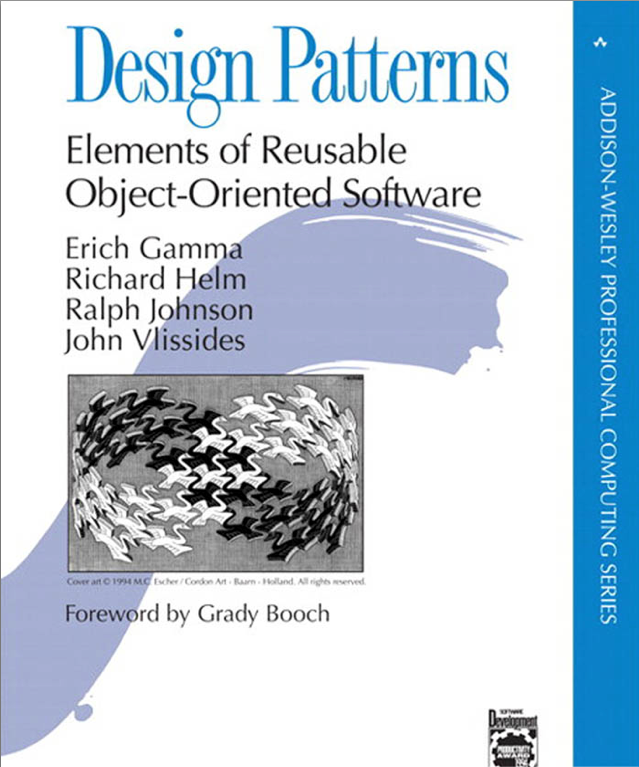
\includegraphics[width=1.9in]{design-patterns-book.png}
\end{center}
\end{column}

\begin{column}{3in}
A recurring object-oriented design.
\begin{itemize}
\item Make proven techniques more accessible to developers of new systems -- don't have to study other systems.
\item Helps in choosing designs that make the system more reusable.
\item Facilitate documenentation and communication with other developers.
\end{itemize}
Design pattern catalog: descriptions of communicating objects and classes that are customized to solve a general design problem in a particular context.

\end{column}

\end{columns}

\end{frame}
%------------------------------------------------------------------------


%------------------------------------------------------------------------
\begin{frame}[fragile]{Elements of Design Patterns}


\begin{itemize}
\item The {\bf pattern name} is a handle we can use to describe a design problem, its solutions, and consequences in a word or two.
\item The {\bf problem} describes when to apply the pattern.
\item The {\bf solution} describes the elements that make up the design, their relationships, responsibilities, and collaborations.  The pattern provides an abstract description of a design problem and how a general arrangement of classes and objects solves it.
\item The {\bf consequences} are the results and trade-offs of applying the pattern.
\end{itemize}


\end{frame}
%------------------------------------------------------------------------

%------------------------------------------------------------------------
\begin{frame}[fragile]{How Design Patterns Solve Design Problems}


\begin{itemize}
\item Finding appropriate objects
\item Determining object granularity
\item Specifying object interfaces
\item Specifying object implementations
\end{itemize}


\end{frame}
%------------------------------------------------------------------------

%------------------------------------------------------------------------
\begin{frame}[fragile]{Types versus Classes}


Class versus interface inheritance
\begin{itemize}
\item An object's class defines how the object is implemented.
\begin{itemize}
\item Class inheritance defines an object's implementaion in terms of another object's implementation.
\end{itemize}
\item An object's type refers to its interface -- the set of methods it can respond to.
\begin{itemize}
\item Interface inheritance is sybtyping.  It describes when an object can be used in place of another.
\end{itemize}
\end{itemize}

\begin{quote}
Program to an interface, not an implementation.
\end{quote}

\end{frame}
%------------------------------------------------------------------------

%------------------------------------------------------------------------
\begin{frame}[fragile]{Reuse Mechanisms}


Inheritance versus composition
\begin{itemize}
\item Inheritance: ``White box reuse''  -- subclass reuses details of superclass and extends with new functionality
\begin{itemize}
\item Defined at compile-time.
\item Straightforward to use
\item ``Inheritace breaks encapsulation'' (superclass implementaiotn exposed to subclasses)
\item Reuse can be difficult in new contexts -- may require rewriting superclasses or carrying baggage.
\end{itemize}
\item Composition: ``Black-box reuse'' -- new functionality obtained by composing objects of other objects
\begin{itemize}
\item Defined at run-time by objects acquiring references to other objects.
\item Must program to interfaces, so interfaces must be well thought-out and stable.
\item Emphasis on interface stability encourages granular objects with single responsiblities.
\end{itemize}
\end{itemize}

\begin{quote}
Favor object composition over class inheritance.
\end{quote}



\end{frame}
%------------------------------------------------------------------------

%------------------------------------------------------------------------
\begin{frame}[fragile]{Designing for Change}


Common causes of redesign (and design patterns that address them):
\begin{itemize}
\item Creating an object by specifying a class explicitly. (Factory)
\item Dependence on specific operations. (Command)
\item Dependence on hardware and software platform. (Factory, Bridge).
\item Dependence on object representations or implementations (Factory, Bridge, Proxy).
\item Algorithmic dependencies. (Visitor, Iterator, Strategy, Template Method)
\item Tight coupling. Design patterns: (Factory, Bridge, Command, Facade, Mediator, Observer).
\item Extending functionality by subclassing.
(Bridge, Chain of Responsibility, Composite, Decorator, Observer, Strategy)
\item Inability to alter classes conveniently. (Adapter, Decorator, Visitor)
\end{itemize}


\end{frame}
%------------------------------------------------------------------------

%------------------------------------------------------------------------
\begin{frame}[fragile]{Selecting a Design Pattern}


\begin{itemize}
\item Consider how design patterns solve design problems.
\item Scan Intent sections.  Read through each pattern's intent to find one or more that sound relevant to your problem. 
\item Study how patterns interrelate.  Studying these relationships can help direct you to the right pattern or group of patterns.
\item Study patterns of like purpose. 
\item Examine a cause of redesign, look at the patterns that help you avoid the causes of redesign.
\item Consider what should be variable in your design. This approach is the opposite of focusing on the causes of redesign. Instead of considering what might force a change to a design, consider what you want to be able to change without redesign. The focus here is on encapsulating the concept that varies, a theme of many design patterns.
\end{itemize}


\end{frame}
%------------------------------------------------------------------------

%------------------------------------------------------------------------
\begin{frame}[fragile]{Using Design Patterns (1 of 2)}


\begin{itemize}
\item Read the pattern once through for an overview.
\item Go back and study the Structure, Participants, and Collaborations sections. Make sure you understand the classes and objects in the pattern and how they relate to one another.
\item Look at Sample Code to see a concrete example of the pattern in code.
\item Choose names for pattern participants that are meaningful in the application context. OK to use abstract participant names from design pattern. For example, if you use the Strategy pattern for a text compositing algorithm, then you might have classes SimpleLayoutStrategy or TeXLayoutStrategy.
\end{itemize}


\end{frame}
%------------------------------------------------------------------------

%------------------------------------------------------------------------
\begin{frame}[fragile]{Using Design Patterns (2 of 2)}


\begin{itemize}
\item Define the classes. Declare their interfaces, establish their inheritance relationships, and define the instance variables that represent data and object references. Identify existing classes in your application that the pattern will affect, and modify them accordingly.
\item Define application-specific names for operations in the pattern. Use the responsibilities and collaborations associated with each operation as a guide. Be consistent in your naming conventions. For example, you might use the "Create-" prefix consistently to denote a factory method.
\item Implement the operations to carry out the responsibilities and collaborations in the pattern. The Implementation section from a pattern catalog and sample code offers hints to guide you in the implementation.
\end{itemize}


\end{frame}
%------------------------------------------------------------------------

%------------------------------------------------------------------------
\begin{frame}[fragile]{Common Design Patterns}

\begin{itemize}
\item {\bf Abstract Factory} Provide an interface for creating families of related or dependent objects without specifying their concrete classes. (GoF, 87)
\item {\bf Factory Method} Define an interface for creating an object, but let subclasses decide which class to instantiate. Factory Method lets a class defer instantiation to subclasses. (GoF, 107)
\item {\bf Adapter} Convert the interface of a class into another interface clients expect. Adapter lets classes work together that couldn't otherwise because of incompat ible interfaces. (GoF, 139)
\item {\bf Composite} Compose objects into tree structures to represent part-whole hierarchies. Composite lets clients treat individual objects and compositions of objects uniformly. (GoF, 163)
\end{itemize}


\end{frame}
%------------------------------------------------------------------------

%------------------------------------------------------------------------
\begin{frame}[fragile]{Common Design Patterns}

\begin{itemize}
\item {\bf Decorator} Attach additional responsibilities to an object dynamically. Decorators provide a flexible alternative to subclassing for extending functionality. (GoF, 175)
\item {\bf Observer} Define a one-to-many dependency between objects so that when one object changes state, all its dependents are notified and updated automatically. (GoF, 293)
\item {\bf Strategy} Define a family of algorithms, encapsulate each one, and make them interchangeable. Strategy lets the algorithm vary independently from clients that use it. (GoF, 315)
\item {\bf Template Method} Define the skeleton of an algorithm in an operation, deferring some steps to subclasses. Template Method lets subclasses redefine certain steps of an algorithm without changing the algorithm's structure. (GoF, 325)
\end{itemize}

\end{frame}
%------------------------------------------------------------------------



% %------------------------------------------------------------------------
% \begin{frame}[fragile]{}


% \begin{lstlisting}[language=Java]

% \end{lstlisting}

% \begin{itemize}
% \item
% \end{itemize}


% \end{frame}
% %------------------------------------------------------------------------


\end{document}
